\subsection{直线和平面垂直的判定与性质}\label{subsec:1-9}

如图 \ref{fig:ltjh-1-24},将书打开直立在桌面 $\alpha$ 上。
观察书的书脊 $AB$ 和各页与桌面的交线的位置关系,显然,它们都是垂直的。
$AB$ 和桌面 $\alpha$ 的位置关系,给我们以直线和平面垂直的形象。

\begin{figure}[htbp]
    \centering
    \begin{minipage}[b]{7cm}
        \centering
        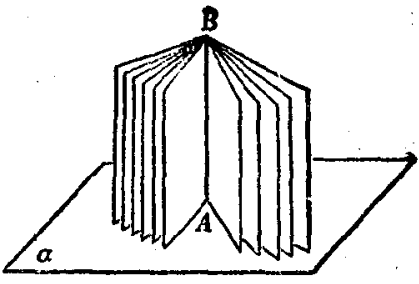
\includegraphics[width=6cm]{../pic/ltjh-ch1-24.png}
        \caption{}\label{fig:ltjh-1-24}
    \end{minipage}
    \qquad
    \begin{minipage}[b]{7cm}
        \centering
        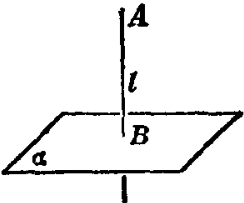
\includegraphics[width=4cm]{../pic/ltjh-ch1-25.png}
        \caption{}\label{fig:ltjh-1-25}
    \end{minipage}
\end{figure}

如果一条直线和一个平面内的任何一条直线都垂直,我们说\zhongdian{这条直线和这个平面互相垂直},
直线叫做\zhongdian{平面的垂线},平面叫做\zhongdian{直线的垂面}。
过一点有且只有一条直线和一个平面垂直;\mylabel{d-zx-pm}
过一点有且只有一个平面和一条直线垂直。\mylabel{d-pm-zx}
平面的垂线和平面一定相交,交点叫做\zhongdian{垂足}。

画直线和水平平面垂直时,要把直线画成和表示平面的平行四边形的横边垂直,
如图 \ref{fig:ltjh-1-25} 中的 $AB$。

直线 $l$ 和平面 $\alpha$ 互相垂直,记作 $l \perp \alpha$。

判定直线和平面垂直,除根据定义外,还有下面的定理:

\begin{dingli}[直线和平面垂直的判定定理][dl:zxhpmcz-pd]
    如果一条直线和一个平面内的两条相交直线都垂直,那么这条直线垂直于这个平面。
\end{dingli}

已知:$m \subset \alpha$, $n \subset \alpha$, $m \cap n = B$, $l \perp m$,  $l \perp n$。

求证: $l \perp \alpha$。

\zhengming 设 $g$ 是平面 $\alpha$ 内的任意一条直线。
要证明 $l \perp \alpha$,根据定义,只要证明 $l \perp g$ 就可以了。

先证明 $l$、$g$ 都通过点 $B$ 的情况(图 \ref{fig:ltjh-1-26})。

在直线 $l$ 上点 $B$ 的两侧分别取点 $A$、$A'$, 使 $AB = A'B$。
那么直线 $m$、$n$ 都是线段 $AA'$ 的垂直平分线,
为了证明 $l \perp g$,可证明直线 $g$ 也是线段 $AA'$ 的垂直平分线。

当 $g$ 与 $m$(或 $n$)重合时,根据已知 $l \perp m$(或$n$),可知 $l \perp g$ 成立。
当 $g$ 与 $m$、$n$ 都不重合时,在平面 $\alpha$ 内作一条直线 $CD$,
与直线 $m$、$n$、$g$ 分别交于点 $C$、$D$、$E$。
连结 $AC$、$A'C$、$AD$、$A'D$、$AE$、$A'E$。则有
$$ AC = A'C \douhao  AD = A'D \douhao $$

% TODO: 暂时没有想到好的方式,这里采用手工调整空白的方式对齐
$\therefore$ \hspace{5cm} $\triangle ACD \quandeng \triangle A'CD$,\\
得 \hspace{5.7cm} $\angle ACE = \angle A'CE$。

$\therefore$ \hspace{5cm} $\triangle ACE \quandeng \triangle A'CE$,\\
得 \hspace{5.7cm} $AE = A'E$,

$\therefore$ \quad $g$ 是 $AA'$ 的垂直平分线。

$\therefore$ \hspace{5cm} $l \perp g$。

如果直线 $l$、$g$ 中有一条或两条不经过点 $B$,那么可过点 $B$ 引它们的平行直线,
由于过点 $B$ 的这样两条直线所成的角就是直线 $l$ 与 $g$ 所成的角,
同理可证这两条直线垂直。因而 $l \perp g$。

综上所述可得
$$ l \perp \alpha \juhao$$

\begin{figure}[htbp]
    \centering
    \begin{minipage}[b]{7cm}
        \centering
        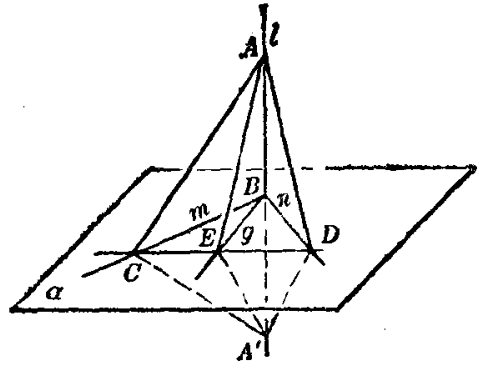
\includegraphics[width=6cm]{../pic/ltjh-ch1-26.png}
        \caption{}\label{fig:ltjh-1-26}
    \end{minipage}
    \qquad
    \begin{minipage}[b]{7cm}
        \centering
        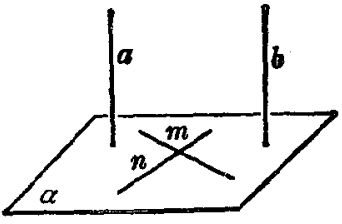
\includegraphics[width=4cm]{../pic/ltjh-ch1-27.png}
        \caption{}\label{fig:ltjh-1-27}
    \end{minipage}
\end{figure}

\liti \zhongdian{如果两条平行直线中的一条垂直于一个平面,那么另一条也垂直于同一个平面。}

已知: $a \pingxing b$, $a \perp \alpha$(图 \ref{fig:ltjh-1-27}).

求证: $b \perp \alpha$。

\zhengming 在平面 $\alpha$ 内作两条相交直线 $m$、$n$。

\jiange
$\left.\begin{aligned}
    a \perp \alpha  \tuichu & \left\{\begin{aligned}
        a \perp m \\
        a \perp n
    \end{aligned}\right. \\
    & \hspace{1.5em} b \pingxing a
\end{aligned}\right\}  \tuichu  \left\{\begin{aligned}
    b \perp m \\
    b \perp n
\end{aligned}\right\}  \tuichu  b \perp \alpha \juhao$
\jiange

下面研究直线和平面垂直的性质。

设 $a \perp \alpha$, $b \perp \alpha$,我们来研究直线 $a$ 和 $b$ 是否平行(图 \ref{fig:ltjh-1-28})。

假定 $b$ 与 $a$ 不平行。

设 $b \cap a = O$, $b'$ 是经过点 $O$ 与直线 $a$ 平行的直线,
平面 $\beta$ 经过直线 $b$ 与 $b'$, $\alpha \cap \beta = c$。

$\because$ \quad $a \perp \alpha$, $b \perp \alpha$,

$\therefore$ \quad $a \perp c$, $b \perp c$。

又 $\because$ \quad $b' \pingxing a$,

$\therefore$ \quad $b' \perp c$。

这样在平面 $\beta$ 内,经过直线 $c$ 上同一点 $O$ 就有两条直线
$b$、 $b'$ 与 $c$ 垂直,这是不可能的。

因此, $b \pingxing a$。

由此,我们得到:

\begin{dingli}[直线和平面垂直的性质定理][dl:zxhpmcz-xz]
    如果两条直线同垂直于一个平面,那么这两条直线平行。
\end{dingli}

从平面外一点引一个平面的垂线,这个点和垂足间的距离叫做\zhongdian{这个点到这个平面的距离}。

\begin{figure}[htbp]
    \centering
    \begin{minipage}[b]{7cm}
        \centering
        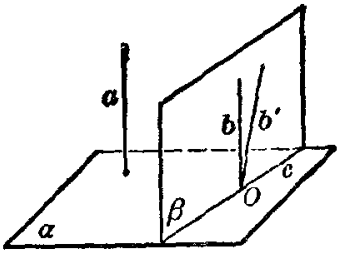
\includegraphics[width=4cm]{../pic/ltjh-ch1-28.png}
        \caption{}\label{fig:ltjh-1-28}
    \end{minipage}
    \qquad
    \begin{minipage}[b]{7cm}
        \centering
        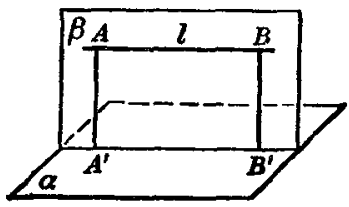
\includegraphics[width=4cm]{../pic/ltjh-ch1-29.png}
        \caption{}\label{fig:ltjh-1-29}
    \end{minipage}
\end{figure}

\liti 已知一条直线 $l$ 和一个平面 $\alpha$ 平行。

求证: 直线 $l$ 上各点到平面 $\alpha$ 的距离相等(图 \ref{fig:ltjh-1-29})。

\zhengming 过直线 $l$ 上任意两点 $A$、$B$ 分别引平面 $\alpha$ 的垂线 $AA'$、$BB'$,垂足分别为 $A'$、$B'$。

$\because$ \quad $AA' \perp \alpha$, $BB' \perp \alpha$,

$\therefore$ \quad $AA' \pingxing BB'$。

设经过直线 $AA'$ 和 $BB'$ 的平面为 $\beta$, $\beta \cap \alpha = A'B'$。

$\because$ \quad $l \pingxing \alpha$,

$\therefore$ \quad $l \pingxing A'B'$。

$\therefore$ \quad $AA' = BB'$。

即直线 $l$ 上各点到平面的距离相等。

一条直线和一个平面平行,这条直线上任意一点到平面的距离,叫做\zhongdian{这条直线和平面的距离}。


\begin{lianxi}

\xiaoti{一条直线垂直于平面内的两条直线,这条直线垂直于这个平面吗?}

\xiaoti{求证:如果三条共点直线两两垂直,那么其中一条直线垂直于另两条直线确定的平面。}

\xiaoti{求证:平面外一点与平面内各点连结的线段中,垂直平面的线段最短。}

\xiaoti{安装日光灯时,怎样才能使灯管和天棚、地板平行?}

\end{lianxi}

